\subsection{Telepresence}

\begin{figure*}
% \begin{center}
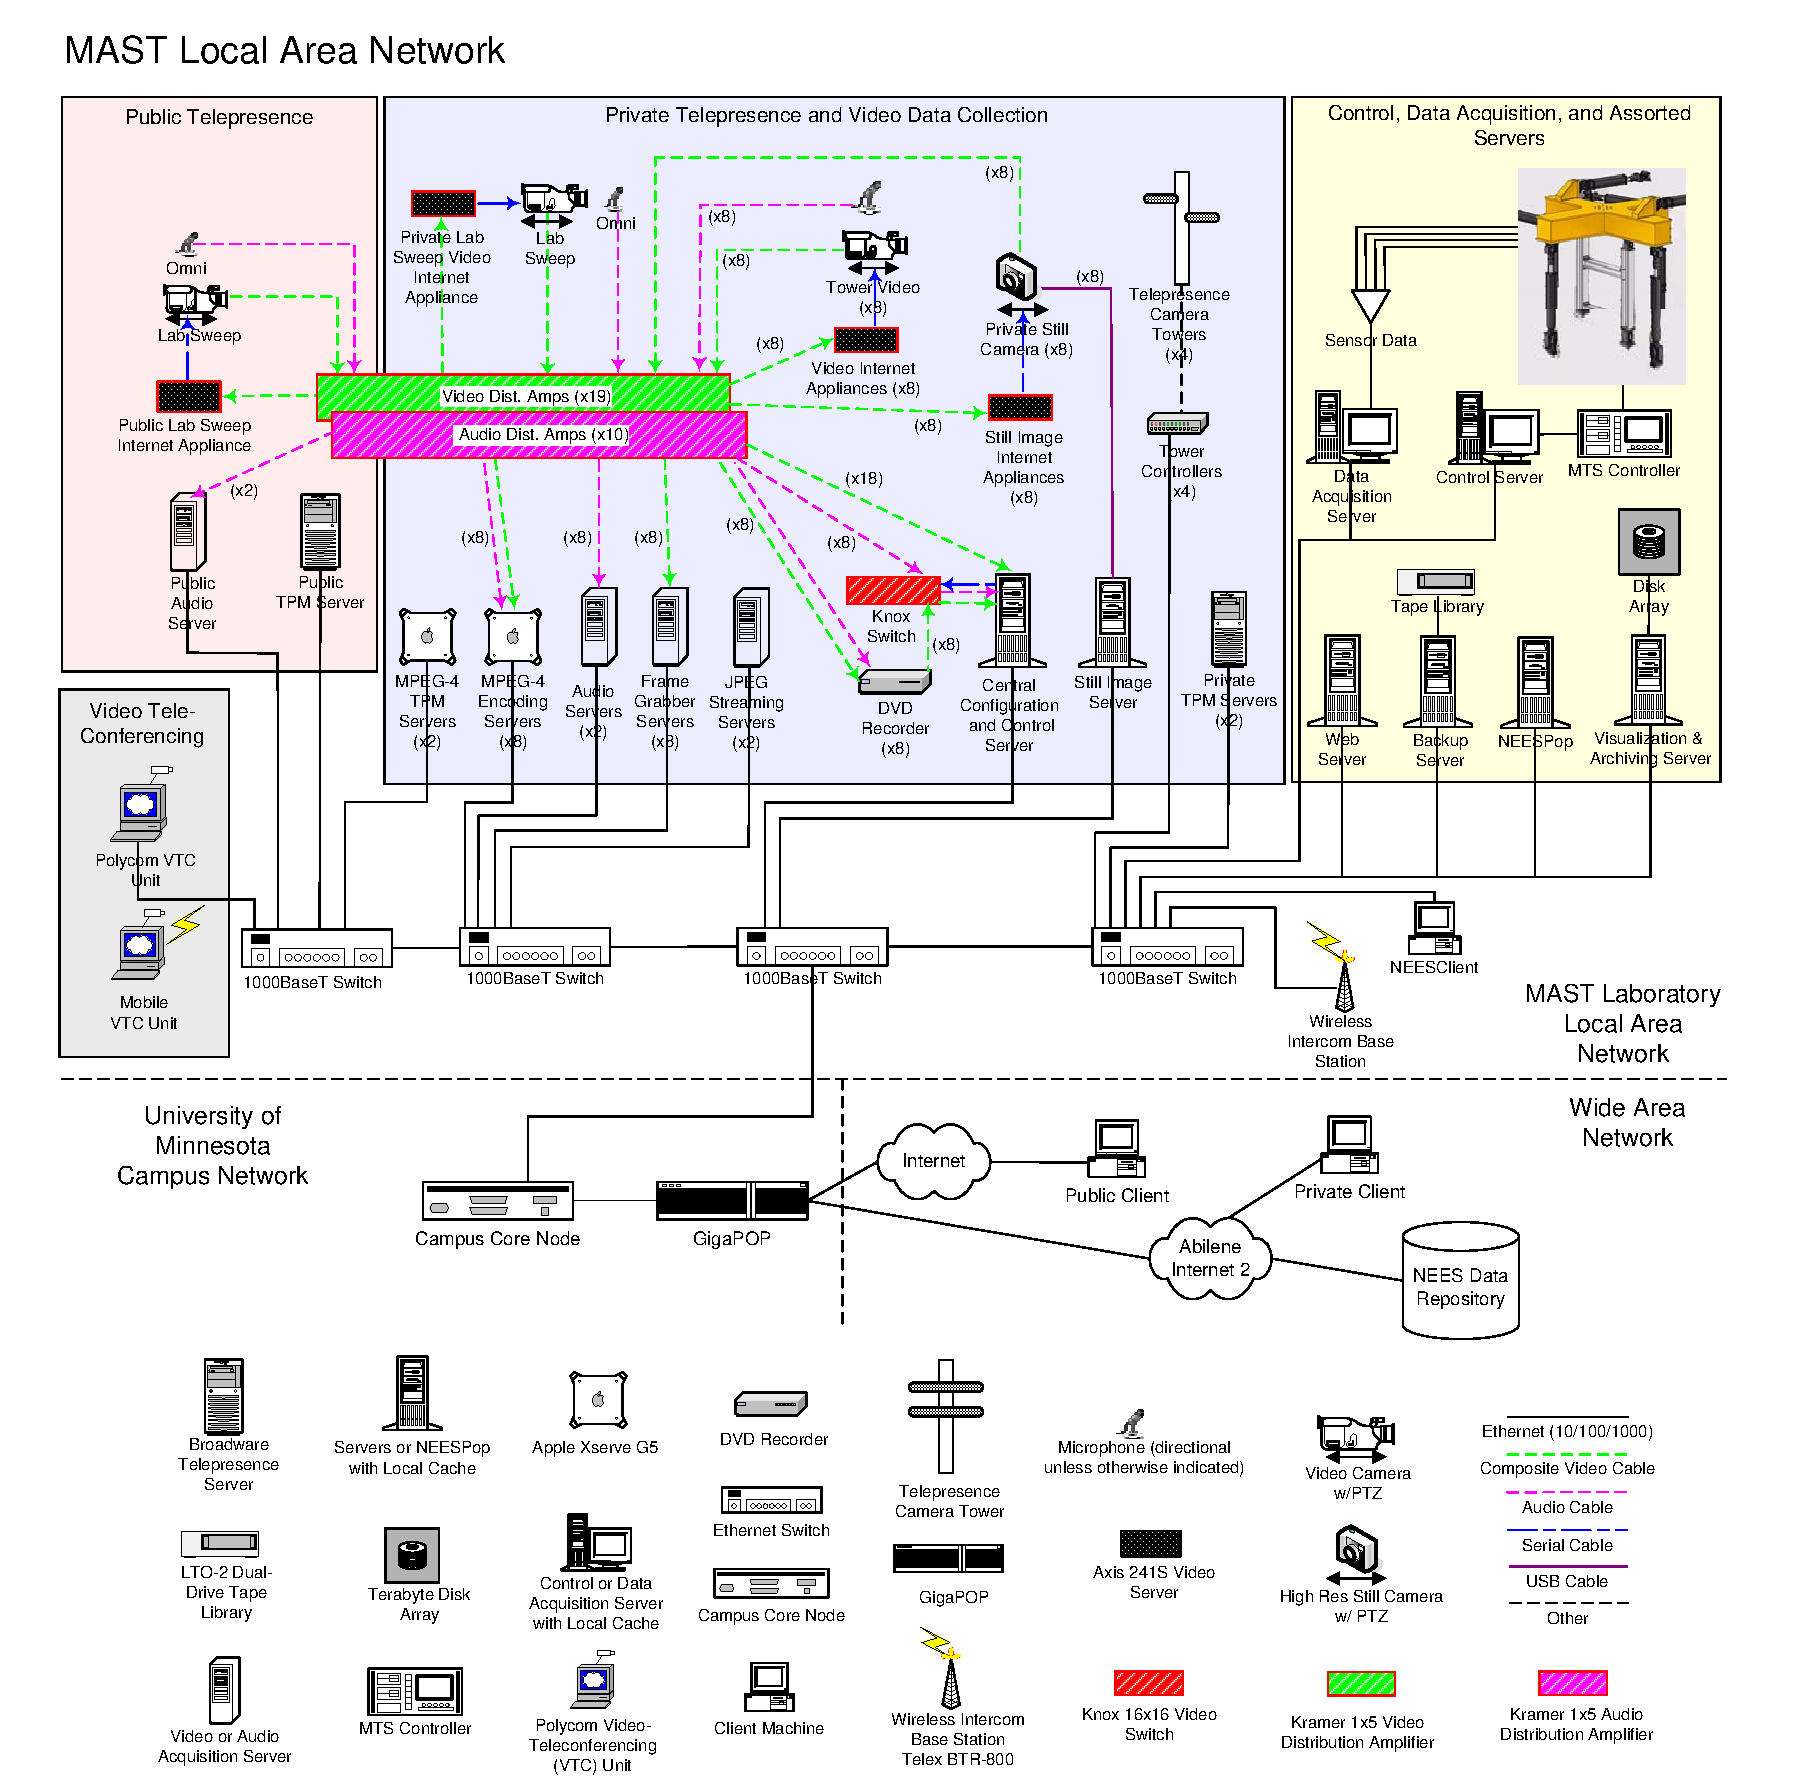
\includegraphics[scale=0.50]{figs/MAST}
% \end{center}
\caption{\label{fig:mast-arch}MAST laboratory network architecture}
\end{figure*}

%(Figure~\ref{fig:ucla-arch})
We deployed RBNB DataTurbine for in a laboratory that conducts Multi-Axial Subassemblage Testing
(MAST) experiments. This is a large-scale test facility, with experiments that may run continuously for a week or more. Experiments are collaborative with remote institutions even spanning multiple countries.
% The MAST (Multi-Axial Subassemblage Testing) lab ~\cite{mast} at the University of Minnesota is a large-scale test facility, with experiments that may run continuously for a week or more. Experiments are collaborative with remote institutions such as the University of Iowa and the University of Puerto Rico at Mayaguez. 
Remote collaboration is thus a requirement and priority. As can be seen in Figure ~\ref{fig:mast-arch}, the local network configuration is extremely complex and highly optimized. 

The MAST lab has 384 channels of data acquisition, running on a National Instruments platform and sampling at 1Hz. This includes data from 256 channel strain gages and 192 channels of voltage inputs (mainly string potentiometers and LVDTs for position measurements). There are eight high-resolution still cameras, one at each corner of the lab floor, mounted on remote-controlled towers. These cameras are used to capture 4 megapixel images of samples as the test progresses, with data annotated by custom code (rewriting the EXIF header) before sending it to the Data Turbine.  Eight of these cameras are on robots, and two permanently mounted with views of the lab floor. There are also ten telepresence (NTSC-resolution) cameras on pan-tilt-zoom (PTZ) platforms to provide remote participants with a sense of the state of the lab and experiment. The camera towers and PTZ cameras also have audio microphones, where the sampled sound is streamed out via the Data Turbine, which accounts for ten channels of audio from the floor. The goal was to deploy RBNB DataTurbine  for data acquisition
from the aforementioned sensors and support streaming with mirroring to remote sites for collaboration. 

\emph{Lessons Learned}

We encountered significant unexpected problems in this experiment. 
\begin{enumerate}
\item NTP was not working properly on all connected systems. This was straightforward to correct.
\item The mirroring to Iowa would fail quickly, with poor performance beforehand. The university campus was using a packet shaper, which decided that RBNB DataTurbine traffic was peer-to-peer file sharing. This meant that RBNB was experiencing more than 70\% packet loss, causing the mirroring to fail. The fix for this required intervention by the % UMN 
campus networking personnel.
\item The % UMN 
Internet2 router was unable to handle the traffic that RBNB generated, and would fail in unpredictable ways. An upgrade was required to solve this.
\item The initial design included multiple machines each hosting an RBNB server; after deployment experience a single quad-CPU (2.8GHz, 4GB RAM) machine running a single RBNB server is used instead. This has sufficient resources and is simpler to administrate and configure. This RBNB server is able to archive about two weeks' worth of data to a 1.2TB RAID array, with all 300+ DAQ channels and video sampled at 1Hz.
\item Java version 1.42 had stability problems, where ten clients would cause problems with server stability. These were resolved in JDK 1.5, and subsequent remote stress testing to another university was problem-free.
\end{enumerate}

The overarching lessons are that data streaming will place unusual demands on the network, and that expertise is required to diagnose and correct the resulting problems. However, once these problems were fixed, we were able to stream data and the system is in production today. 
